% Template for a Computer Science Tripos Part II project dissertation
\documentclass[12pt,a4paper,twoside,openright]{report}

\usepackage[indent=0pt,skip=10pt]{parskip}
\usepackage[pdfborder={0 0 0}]{hyperref}    % turns references into hyperlinks
\usepackage[margin=25mm]{geometry}  % adjusts page layout
\usepackage{graphicx}  % allows inclusion of PDF, PNG and JPG images
\usepackage{verbatim}
\usepackage{docmute}   % only needed to allow inclusion of proposal.tex
\usepackage[utf8]{inputenc}
\usepackage{mathtools}
\usepackage{changepage}
\usepackage{url}
\usepackage{blindtext}
\usepackage[dvipsnames]{xcolor}

%\raggedbottom                           % try to avoid widows and orphans
\sloppy
\clubpenalty1000%
\widowpenalty1000%

\renewcommand{\baselinestretch}{1.1}    % adjust line spacing to make
                                        % more readable
\newcommand{\vital}{\colorbox{BrickRed}{Vital}}
\newcommand{\veryhard}{\colorbox{BrickRed}{Very Hard}}

\newcommand{\hard}{\colorbox{RedOrange}{Hard}}
\newcommand{\high}{\colorbox{RedOrange}{High}}

\newcommand{\medium}{\colorbox{Dandelion}{Medium}}

\newcommand{\low}{\colorbox{LimeGreen}{Low}}
\newcommand{\easy}{\colorbox{LimeGreen}{Easy}}



\begin{document}
%TC:ignore
% Change these

\newcommand{\mcandidate}{2416B}
\newcommand{\mfullname}{Jude Howard-Gluckstein Tyrrell}
\newcommand{\mcollege}{Homerton College}
\newcommand{\mtitle}{Notation for Phonological Audio Composition}
\newcommand{\mexamination}{Computer Science Tripos -- Part II}
\newcommand{\mdate}{May 2023}
\newcommand{\moriginator}{Prof. Alan Blackwell}
\newcommand{\msupervisor}{Prof. Alan Blackwell}
\newcommand{\mwordcount}{10814}
\newcommand{\mlinecount}{0}
% Consent to the dissertation made available to University members
\newcommand{\mconsent}{I am content for my dissertation to be made available to the students and staff of the University.}
% For the Declaration of originality
\newcommand{\msignature}{Jude Tyrrell}


\bibliographystyle{plain}


%%%%%%%%%%%%%%%%%%%%%%%%%%%%%%%%%%%%%%%%%%%%%%%%%%%%%%%%%%%%%%%%%%%%%%%%
% Title


\thispagestyle{empty}

\rightline{\LARGE \textbf{\mfullname}}

\vspace*{60mm}
\begin{center}
\Huge
\textbf{\mtitle} \\[5mm]
\mexamination \\[5mm]
\mcollege \\[5mm]
\mdate  % today's date
\end{center}

%%%%%%%%%%%%%%%%%%%%%%%%%%%%%%%%%%%%%%%%%%%%%%%%%%%%%%%%%%%%%%%%%%%%%%%%%%%%%%
% Proforma, table of contents and list of figures

\pagestyle{plain}

\newpage
\newpage
\section*{Declaration of originality}

I, \mfullname{} of \mcollege, being a candidate for Part II of the Computer Science Tripos, hereby declare that this dissertation and the work described in it are my own work, unaided except as may be specified below, and that the dissertation does not contain material that has already been used to any substantial extent for a comparable purpose. \mconsent

\bigskip
\leftline{Signed \msignature}
\bigskip
\leftline{Date \today}

\chapter*{Proforma}

{\large
\begin{tabular}{ll}
Candidate Number:   & \bf \mcandidate                   \\
Project Title:      & \bf \mtitle                       \\
Examination:        & \bf \mexamination, \mdate         \\
Word Count:         & \bf \mwordcount\footnotemark[1]   \\
Code Line Count:    & \bf \mlinecount                   \\
Project Originator: & \bf \moriginator                  \\
Supervisor:         & \bf \msupervisor                  \\ 
\end{tabular}
}
\footnotetext[1]{This word count was computed
by 
}
\stepcounter{footnote}


\section*{Original Aims of the Project}
% At most 100 words




\section*{Work Completed}
% At most 100 words


\section*{Special Difficulties}
% At most 100 words


\newpage

\tableofcontents

\listoffigures

\newpage
\section*{Acknowledgements}


%%%%%%%%%%%%%%%%%%%%%%%%%%%%%%%%%%%%%%%%%%%%%%%%%%%%%%%%%%%%%%%%%%%%%%%
% now for the chapters

\pagestyle{headings}
%TC:endignore
\chapter{Introduction}
\textit{
Since the development of electronic devices, people have utilised them extensively in the creation of art, especially music. From the theremin to synthesizers to trackers and modern day Digital Audio Workstations (hereafter referred to as DAWs), electronics have enabled people to compose music easier than ever before, and to achieve previously unachievable sounds.
}

This dissertation explores the full capability of modern computers to facilitate particular styles of artistic audio composition. It presents a novel piece of software (tuPAC: Totally Usable Phonological Audio Composer) that (achieves) this goal through a graphical user interface, as evaluated against an industry-standard audio composition tool (elaborate on results), and acts as a notation for these compositions.
 
 The research and development in this project was done with guidance from an artist who is interested in composing music with only vocal sounds, experimenting with the structure of spoken language and the sounds made when speaking in order to create art. For the rest of the dissertation, this will be referred to as phonological composition, as it focuses on the manipulation of the structure of language to create an effect, rather than traditional melodic or rhythmic patterns, although these features may also be incorporated into the music. Note that this is not an established term but one that I am using as it best describes the type of composition that the project caters to, but there exists a history of composition styles which fall under this category throughout Western classical and contemporary music.

\section{Artistic Background}
The isorhythmic motet is a particular style of polyphonic vocal composition which first appeared in 13th century French music \cite{Bent01}, notably used in the work of Machaut. Polyphonic vocal compositions consist of multiple voices singing different melodies. The defining feature of isorhythmic motets is the repetition and augmentation of rhythmic and melodic patterns - referred to in literature as \textit{color} and \textit{talea} - performed as layered vocals. This style is an early example of music which uses structures which are the focus of this dissertation: layering, repetition and augmentation in vocal compositions.

Steve Reich is a prominent contemporary composer most well known for his work in composing minimalist music. His composition Proverb contains 6 voices which recite a short piece of text from Ludwig Wittgenstein \cite{ReichProverb}. It draws from the medieval polyphonic compositions in style, and repeats and augments the quote throughout the piece. Reich splits up a sentence into smaller parts and repeats these parts individually. In another contemporary composition, O King by Luciano Berio, individual syllables of Martin Luther King's name are pronounced and repeated by a voice throughout the piece. In both of these contemporary compositions, the structure of spoken language is broken down and manipulated by the artist.

\section{Motivation}
 The most popular metod of modern digital music production ish certainly the DAW. Popular DAWs like Ableton, FL Studio and Logic Pro are used almost universally in the composition of modern music, and such are a go-to for artists looking to create music through digital means.

 However, as we will see in the preparation chapter, the design of these programs doesn't lend itself to all forms of composition equally, and whilst they work well in general, there certainly is different approaches to software design that would better cater to the needs, in terms of ease of use and efficiency, of specific use cases.


\section{Project summary}
In this project, I:
\begin{enumerate}
    \item Develop a computational model that accurately represents the structures of phonological composition.
    \item Create a text-based tool which demonstrates the essential ideas of the model.
    \item Design a user interface which creates a visual representation of this model.
    \item Implement this interface into software, providing a digital audio composition tool for artists as an alternative to existing tools, supporting a different approach to composition.
\end{enumerate}

Each of these goals were successfully completed and this dissertation presents the results, as evaluated using standard human-computer interaction techniques.

\chapter{Preparation}
This chapter describes the research and preparation that was necessary before the implementation of the text-based and graphical tools. First, we look at what was needed for this project to succeed.

\section{Requirements Analysis}
In the project proposal, four success criteria were set out for this project. Here, these criteria are broken down and realised into specific achievable tasks, along with some additional possible extension tasks.

\begin{table}[h]
    \centering
    \begin{tabular}{|c|c|c|}
        \hline
         Task & Priority & Difficulty \\
         \hline
         Develop model of composition & \vital & \medium \\
         \hline
         \multicolumn{3}{|c|}{Text-based tool capabilities} \\
         \hline
         Play audio & \vital & \easy \\
         Represent model & \vital & \medium \\
         Mapping IPA characters to samples & \medium & \easy \\
         \hline
         \multicolumn{3}{|c|}{Graphical tool capabilites} \\
         \hline
         Play audio loaded from file & \vital & \medium \\
         Represent model & \high & \hard \\
         Ensure time keeping of audio & \high & \hard \\
         Apply effects to audio & \medium & \medium \\
         Neural synthesis integration & \low & \veryhard \\
         \hline
    \end{tabular}
    \caption{Caption}
    \label{tab:req_anal}
\end{table}

Whilst the above tasks are necessary for the project's success, the true success of the project will come from the clarity, usability and efficiency of the interface, for actual users. This success cannot be measured just by the functionality and design choices of the interface, but through user testing, as was carried out in the evaluation stage of the project.  The evaluation measures the projects success in terms of:
\begin{itemize}
    \item Usability: The ability for the program to make the user's life easier by making common actions fast and intuitive.
    \item Clarity: There is a clear correspondence between what happens on the screen, and what the user imagines is happening to their composition. When the user makes a change, the program changes the audio appropriately, how the user expects.
    \item Functionality: The user is not limited in what they are able to do, and can achieve whatever they want to do with the program.
\end{itemize}

\section{Existing Tools}
\subsection{Digital Audio Workstations}
In this dissertation, I will primarily focus on Ableton Live when discussing DAWs, as it is the one I personally have the most experience with and it is commonly used in electronic music production. It is also the DAW used for evaluation against my project.

\begin{figure}[h]
    \centering
    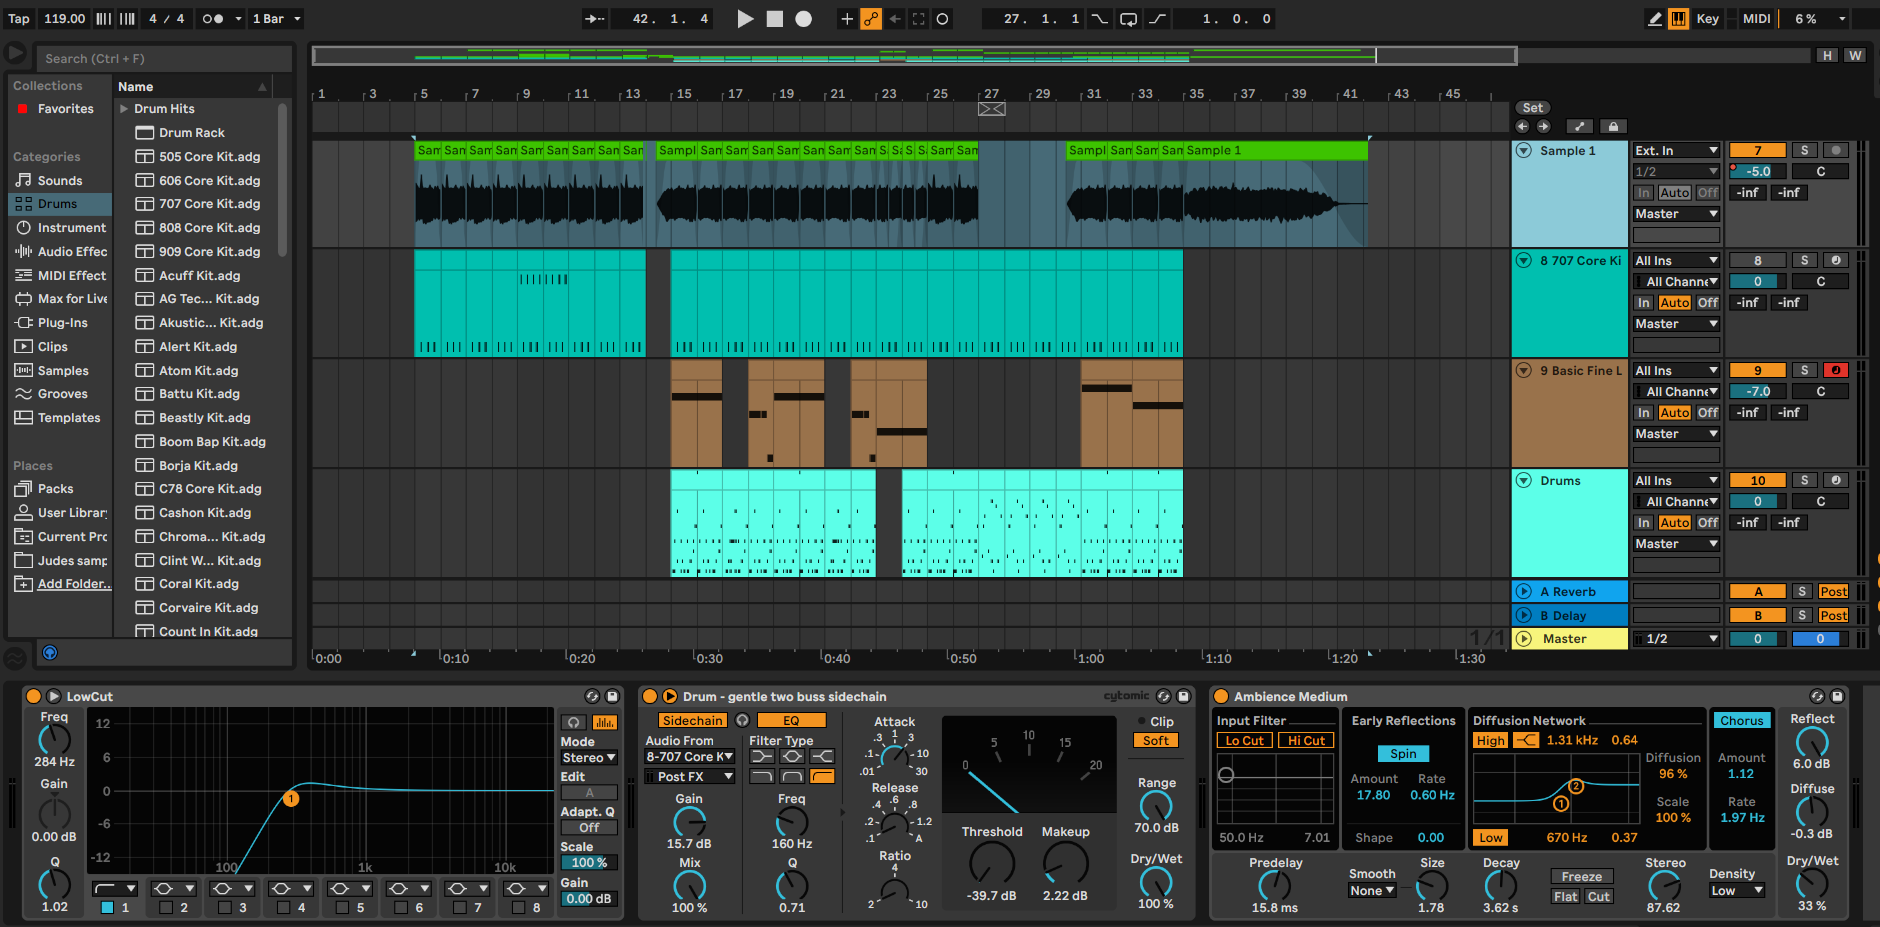
\includegraphics[scale=0.3]{images/ableton example.png}
    \caption{UI of Ableton Live}
    \label{fig:ableton}
\end{figure}

Ableton Live's main interface consists of ``tracks" which can contain either sound clips or MIDI sequences which define the pitches and timing of notes to be digitally generated. The horizontal axis represents time, starting from the left and moving to the right, and the vertical axis generally represents different instruments (separate trakcs), and sometimes pitch. Effects can be added to and parameters adjusted on individual tracks or groups of tracks. 

This structure and design, typical for DAWs, works with an intuition that lines up with traditional composition - each track corresponds to an instrument which can be fed through different effects. Visually, this approach resembles modern staff notation (Figure 2.2), where the horizontal axis represents time, vertical axis represents pitch, and different instruments or parts are placed on separate staffs (collections of 5 horizontal lines).

\begin{figure}[h]
    \centering
    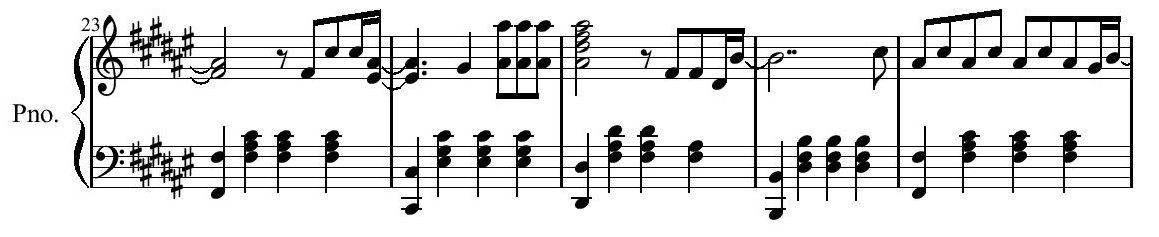
\includegraphics[scale=0.7]{images/modern staff notation.png}
    \caption{Example of modern staff notation}
    \label{fig:my_label}
\end{figure}

This representation of audio is clearly established and will have been encountered by almost all musicians. This is important as users will expect certain features implicitly from all designs, such as the horizontal axis representing the passing of time from left to right.

\subsection{Live Coding}
An existing alternative digital composition style is live coding, a technique used to generate art in real time using a programming language. For music, a popular example is Sonic Pi.

\begin{figure}[h]
    \centering
    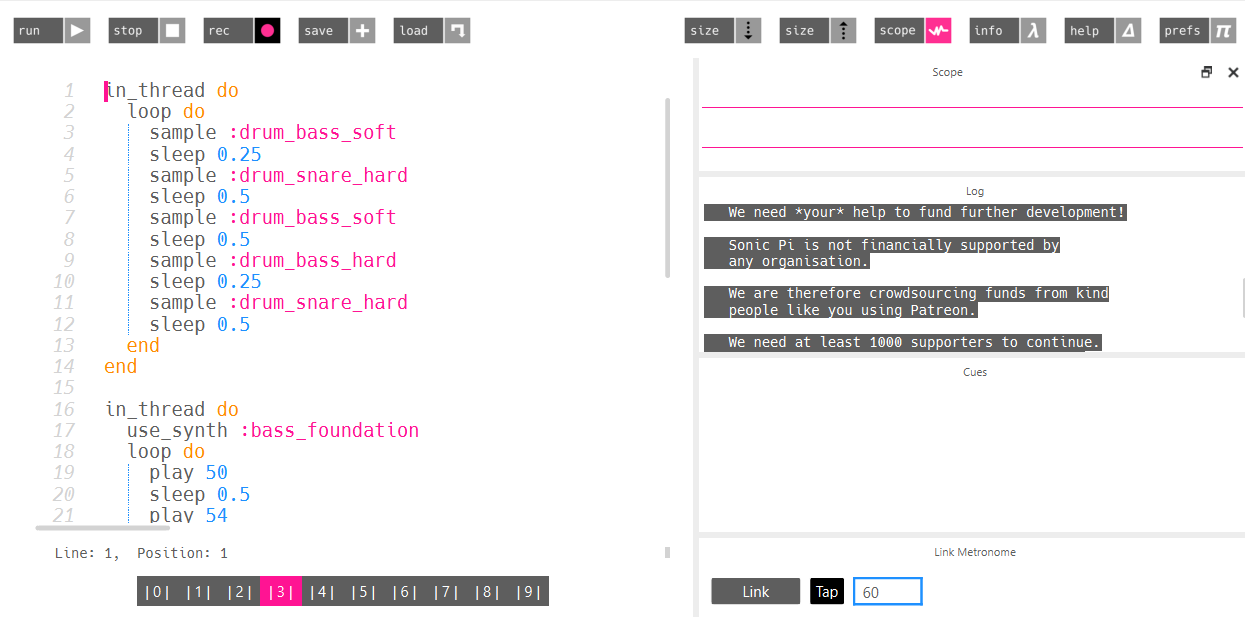
\includegraphics[scale=0.4]{images/sonicpi.png}
    \caption{UI of Sonic Pi}
    \label{fig:sonic_pi}
\end{figure}

Live coding software allows users to generate audio through writing programs, with the defining feature being the ability to modify the code whilst the audio is running and seamlessly change the audio as it is played. This approach to making music is vastly different from industry-standard DAWs, and is often used for performance art.

Live coding platforms differ from DAWs in that there is generally less complex functionality, with more focus on simpler but easier manipulation, particularly the repetition and augmentation of sounds previously defined. This makes the process of live coding plausible in real time whilst still sounding good. This approach is much closer to the goal of this project, and so was a primary focus of research and preparation.

\section{Sonic Pi and Strudel}
In preparation for the development of the project, I researched two live coding platforms in order to build my text tool using the framework of one of them.

Sonic Pi is written in C++ and Ruby. The GUI is written in C++ whilst the code parsing and audio generation is done in Ruby. It synthesises audio by sending OSC (Open Sound Control) messages to SuperCollider, which keeps track of all synthesisers, samples and effects being triggered by the Sonic Pi interface. The codebase is large but it has an API meaning that one could develop their own platform and use the Ruby portion of the software to generate sound using SuperCollider easily without the C++ GUI.

Strudel is a web-based live coding platform built in Javascript, based on another live coding language called TidalCycles. It mainly uses the Web Audio through a framework called Tone.js to synthesise audio, and was still in an experimental stage of development at the time of this project being researched. The software is relatively small, and the codebase easy to navigate and manipulate, as it is written in a modular style that splits up different parts of the software into separate packages which can be used individually.

I decided to continue my research using the Sonic Pi platform, as Strudel is too incomplete in its current form to work with and could cause additional difficulties down the line.

\section{Software Engineering}
\subsection{Framework}
As mentioned, Sonic Pi was used to develop the text tool as it provided the necessary features for its demonstrative purposes.

Electron was chosen as the framework for the graphical tool. Electron builds web pages written in HTML, CSS and Javascript as desktop applications using Chromium and Node.js. Naturally, npm was used as the package manager as is default with Node.js software. 

\subsection{Programming Languages}
The text tool was written in the Sonic Pi GUI, in Sonic Pi's own language, which is essentially Ruby.

After research into both Javascript and Typescript, it was decided to write the project in Typescript, which is an extension of the Javascript language which allows static type checking, and transpiles into Javascript code. It also adds a few features that make object oriented programming easier, which was deemed valuable to the project.

\subsection{Libraries}
\subsubsection{Audio}
I considered using SuperCollider directly with my project, but eventually decided not to use it. SuperCollider is extremely powerful, but could cause a lot of implementation issues due to its complexity. There is a library available for Javascript named supercollider.js, but even with this library, the complexity of SuperCollider would be a considerable difficulty in the implementation of my tool, and the added functionality and modularity over simpler audio libraries is not necessary for my project.

Tone.js is a Web Audio framework which supplies an API for audio applications written in Javascript. It supplies reliable event scheduling, audio playback from files and a system for linking effects and sounds together, and through to output. The features supplied by this library are sufficient for this project, and should be easy to implement, so was chosen for the time-keeping and audio playback of the graphical tool. It is also used in Strudel as one of the main options for audio generation. Based on the ease of implementation, and established widespread usage, this library was chosen for my project.

\subsubsection{Visual Interface}
For the graphical interface, I needed a platform that was as powerful as possible to support my development, but malleable enough to accurately represent the design of the tool.


\subsection{Development Methodology}

\section{Starting Point}
\subsection{Text tool}
The text tool was built in Sonic Pi's own language, which handles everything from audio generation to time keeping. As the text tool was only for demonstration to the user and exploration of possible useful features, this was sufficient. I have only briefly used Sonic Pi prior to this project and was required to learn its native language, which is based on the programming language Ruby, which I have also never used before.

\subsection{Graphical tool}
The graphical tool for the project was built using Electron and Node.js, and written in Typescript. The sound was generated using the Tone.js library, which has a reliable time-keeping system. I have never used Javascript, Typescript, Electron, Node.js or Tone.js in any previous work. The graphical interface was rendered using p5.js which is able to render text, shapes and lines onto a HTML canvas. I have previously used the Python version of p5.js, Processing, which is very similar to the Javascript library.


\chapter{Implementation}
\section{Computational Model of Composition}

\section{Text-based tool}

\section{tuPAC}
\subsection{Repository overview}



\subsection{Waveforms}

\subsection{Time Bar Translation}

\chapter{Evaluation}



\chapter{Conclusions}
\section{Project Summary}
The project was successful. A novel system was designed and developed which provides an alternative to modern composition techniques which improves the digital composition process for particular styles of composition, particularly those which utilise the layering, repetition and augmentation of parts of speech. The functionality and design of the system were decided with input from an artist interested in phonological composition and the final result accurately reflected what they wanted from such a system.

\section{Further Work}
The system that has been developed is somewhat lacking in features due to the limited scope of the project and difficulty of certain desired functionality. This project has provided the theoretical and practical basis for further exploration into the potential of audio composition interfaces and their ability to assist in the creation of music.
%TC:ignore
%%%%%%%%%%%%%%%%%%%%%%%%%%%%%%%%%%%%%%%%%%%%%%%%%%%%%%%%%%%%%%%%%%%%%
% the bibliography
\addcontentsline{toc}{chapter}{Bibliography}
\bibliography{refs}

%%%%%%%%%%%%%%%%%%%%%%%%%%%%%%%%%%%%%%%%%%%%%%%%%%%%%%%%%%%%%%%%%%%%%
% the appendices
\appendix

\chapter{Latex source}

\section{metadata.tex}
{\scriptsize\verbatiminput{metadata.tex}}

\section{main.tex}
{\scriptsize\verbatiminput{main.tex}}

\section{proposal.tex}
{\scriptsize\verbatiminput{proposal.tex}}

\chapter{Makefile}

\section{makefile}\label{makefile}
{\scriptsize\verbatiminput{makefile.txt}}

\section{refs.bib}
{\scriptsize\verbatiminput{refs.bib}}


\chapter{Project Proposal}

\documentclass{article}
\usepackage[utf8]{inputenc}
\usepackage{graphicx}
\usepackage[indent=0pt,skip=10pt]{parskip}
\usepackage[a4paper, total={6in,8in}]{geometry}

\begin{document}

\section*{Introduction}

There exists a wide variety of digital tools to aid the composition of music. Modern DAWs (Digital Audio Workstations) such as Ableton and Fruity Loops are used extensively in the recording, mixing and mastering of most of the music that is produced today. These applications are designed to allow musicians to easily rearrange, layer and manipulate snippets of audio which can be imported from external sources, recorded onto the tracks or generated by MIDI instruments. While this design makes musical composition and recording simple and accessible for many popular styles of music, it can be restricting to other styles of composition and inhibit explorations into more niche musical expressions. 
\begin{figure}[h]
    \centering
    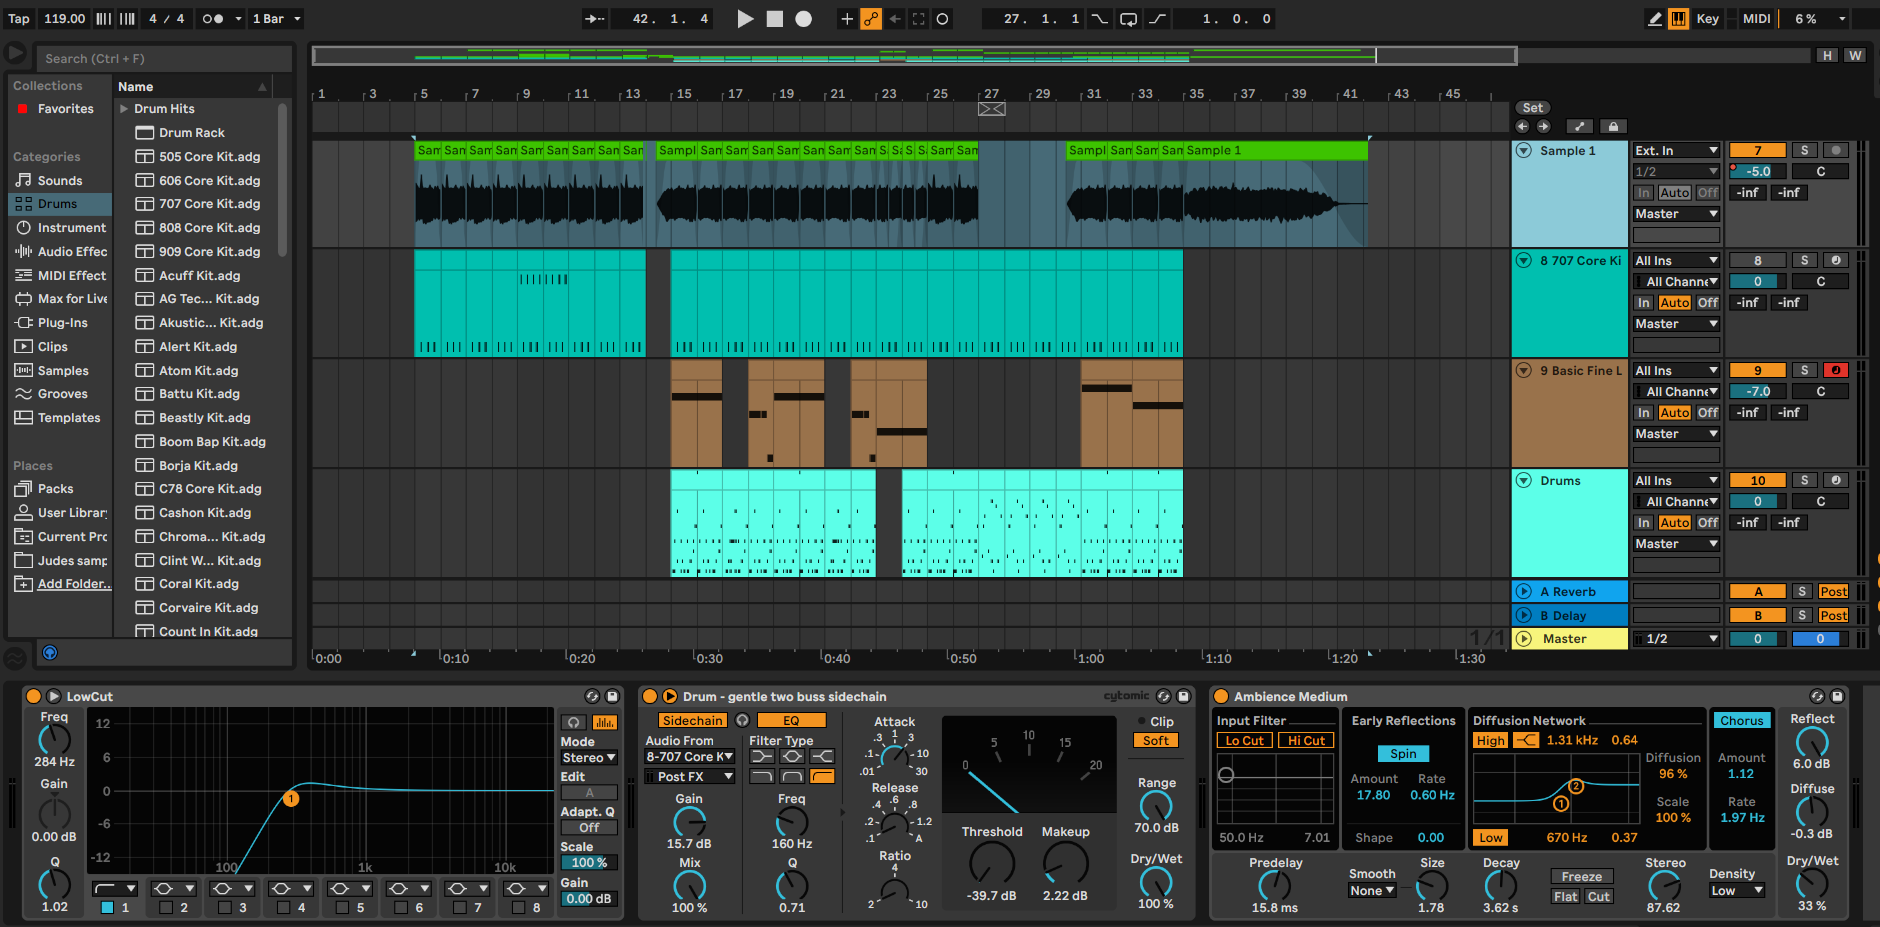
\includegraphics[scale=0.3]{images/ableton example.png}
    \caption{An example of an industry-standard DAW (Ableton 11)}
    \label{fig:ableton}
\end{figure}

Another style of digital music composition that is particularly relevant to my project is through live coding techniques. Live coding (with regards to musical composition) is a performance art in which the artist types code in front of an audience, into an environment which translates the code into music.

TidalCycles is one such platform. Tidal is software which allows people to create music through programming. Users create rhythmic patterns and generate sounds from synths or play samples as dictated by these patterns. It is embedded in the Haskell programming language and uses a custom synth and sampler called SuperDirt, built on the SuperCollider platform.

For my project, I will create an interactive music composition tool which facilitates the composition of music using speech sounds. These sounds may be generated digitally or from small samples of real recordings. I will build a text-based tool on top of an existing text-based audio generation platform (Strudel or Sonic Pi) which will allow users to create music from small literals representing snippets of speech, as well as a graphical user interface which allows users to rearrange and connect blocks to generate audio, in a style similar to the popular visual programming language Scratch.

Strudel is a web-based live coding environment intended to replicate the ideas of TidalCycles, but instead built on JavaScript and run in a browser. It uses a few different browser-available playback methods, most notably the Web Audio API and Tone.JS. There is a work-in-progress feature which allows it to communicate with SuperCollider and run SuperDirt.
\begin{figure}[ht]
    \centering
    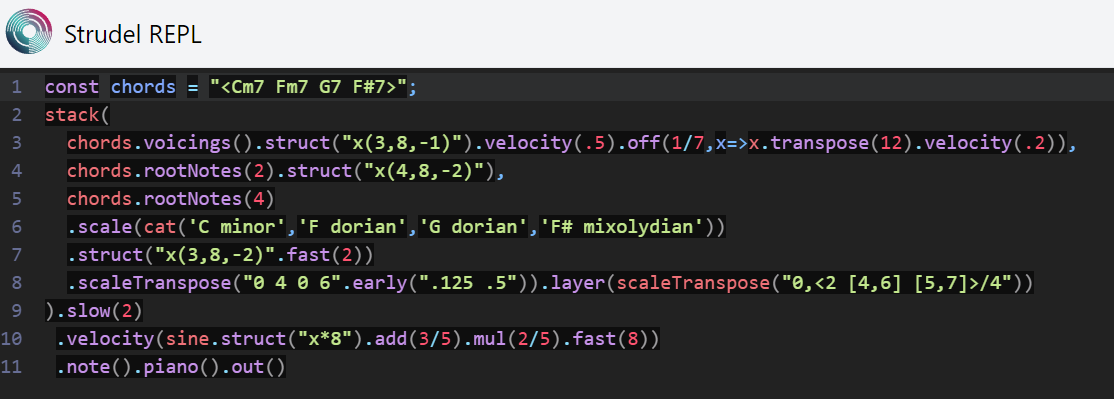
\includegraphics[scale=0.5]{images/strudel.png}
    \caption{The Strudel REPL (web-based application which runs Strudel), with example code/music}
    \label{fig:strudel}
\end{figure}

Another example of a live coding platform that I could work with is Sonic Pi, which is a standalone application with a much simpler language to write music and more in-depth tools than Strudel, but it is more limiting in the ease of expressiveness of the language. It is written in C++ and Ruby. It also uses SuperCollider to generate audio.
\section*{Starting Point}
I have very little experience with live coding and digital audio generation. I have no experience working in JavaScript or Ruby. I will need to learn about how Strudel and Sonic Pi work during the project, and will need to learn how to work with JavaScript or Ruby.
\section*{Substance of Project}
\subsection*{Core}
I will produce a piece of software which allows users to write code and generate audio from speech sounds in order to create music. Users will be able to take small snippets of speech and combine them by playing them back in a chosen order, with a chosen rhythm, by layering them, and by manipulating them in various ways.

I will also produce a piece of software which allows user to achieve a similar goal through diagrammatic means. A GUI will allow a user to take small speech literals as blocks and order them, pass them through filters, layer them or loop them.

Although tools exist that already allow you to do what my project will achieve, it will greatly improve the efficiency for a style of composition which, to my knowledge, has no tools dedicated to enabling it. You can achieve what my project will achieve in a standard DAW, but my tool will allow users to achieve more complicated rhythms and structures in much less time than they would moving samples of speech around in a DAW. It also makes the process much more accessible, allowing users with little experience working with digital composition tools or with programming to work with this style of proposition and to work with live coding techniques.
\subsection*{Extensions}
Some possibles extensions of my project would:
\begin{itemize}
    \item Build an explicit formal language describing the composition and generation of audio, based on the text-based tool.
    \item Change the text-based tool to reflect the definition of the formal language.
    \item Change the graphical tool to represent this formal language.
    \item Integrate neural synthesis of speech sounds into my composition tool. Antoine Caillon and Philippe Esling released a paper last year detailing a variational auto-encoder they have developed (RAVE) which allows for fast, high quality audio synthesis. I could implement RAVE into the tool to allow users to generate their own speech audio with state-of-the-art neural synthesis, adjusting parameters to change the sound in real time.
\end{itemize}
\section*{Success Criterion}
In order to have succeeded in my project, I require:
\begin{itemize}
    \item Software which allows users to write code which will use speech sounds to generate an audio output.
    \item Software which allows users to rearrange blocks specifying speech sounds and operations on those sounds in order to generate an audio output.
    \item Both pieces of software should allow for users to:
    \begin{itemize}
        \item Play back a small sample of speech.
        \item Arrange multiple sounds to be played back with a particular rhythm and order.
        \item Layer multiple sounds to be played alongside each other.
        \item Manipulate sounds with filters and effects.
    \end{itemize}
    \item The software be evaluated against an industry-standard DAW in user tests to express the efficacy of both the graphical and text-based tool in the production of phonological music.
\end{itemize}
For the final bullet point, I will supply the software to users who will give written feedback on the ease of use of my tool and existing tools. I will also measure the time taken for users to complete specific tasks to measure quantitatively the improvement on certain tasks over existing tools. I will use A/B testing to compare the two implementations, text-based and graphical, to measure the ease of use for each tool.
\section*{Timetable}
\subsection*{Feedback}
Over the duration of my project, I plan to interact with users for feedback. I am already in contact with one artist and I will venture to find other possible users of my tool through people I know and get feedback from a wider source. In the first few weeks, I will need to fill in the form for the Ethics Committee to approve the involvement of human participants.
\subsection*{Week 1/2: 16th Oct. - 29th Oct.}
\begin{itemize}
    \item Study Strudel framework.
    \item Study Sonic Pi framework.
    \item Set up work environment for development of text-based tool.
\end{itemize}
{
\centering\textbf{Milestone:} Decide whether to work with Strudel or Sonic Pi, supplying a report describing the details of the research and my choice to my supervisor. Be able to compile and run Strudel and/or Sonic Pi on my own machine, allowing for my own modifications and additions to the code.
}
\subsection*{Week 3/4: 30th Oct. - 12th Nov.}
\begin{itemize}
    \item Research system for generation of audio.
    \item Understand how to generate, combine and manipulate audio to produce new outputs.
\end{itemize}
{
\centering\textbf{Milestone:} Write program which is able to generate sample audio outputs, working on samples given by user.
}
\subsection*{Week 5/6: 13th Nov. - 26th Nov.}
\begin{itemize}
    \item Begin programming of text-based composition tool.
\end{itemize}
{
\centering\textbf{Milestone:} Have functioning text-based tool which allows users to input code and generate audio using small snippets of speech.
}
\subsection*{Week 7/8: 27th Nov. - 10th Dec.}
\textit{Michaelmas term ends: 1st Dec. Varsity skiing trip}
\begin{itemize}
    \item Continue work on text-based tool.
    \item Test text-based implementation on user, get feedback.
\end{itemize}
{
\centering\textbf{Milestone:} Report describing user feedback, possible improvements and tweaks to system.
}
\subsection*{Week 9/10: 11th Dec. - 24th Dec.}
\begin{itemize}
    \item Refine text-based tool based on feedback.
\end{itemize}
{
\centering\textbf{Milestone:} New, improved version of tool modified based on the feedback from the user.
}
\subsection*{Week 11/12: 25th Dec. - 7th Jan.}
\textit{Christmas and New Years Eve, will not be completing much work.}
\begin{itemize}
    \item Research libraries for creating visual programming languages (e.g. Blockly).
\end{itemize}
{
\centering\textbf{Milestone:} Write up a page for project supervisor describing what I have learnt, what library I will use and how I will use the library to create a GUI.
}
\subsection*{Week 13/14: 8th Jan. - 21st Jan.}
\textit{Lent term starts: 17th Jan.}
\begin{itemize}
    \item Build diagrammatic tool for phonological audio composition.
\end{itemize}
{
\centering\textbf{Milestone:} Working GUI, allowing users to rearrange blocks in order to generate audio in different ways.
}
\subsection*{Week 15/16: 22nd Jan. - 4th Feb.}
\textit{Progress deadline due: 3rd Feb (12pm)}
\begin{itemize}
    \item Feedback from user.
    \item Improve on GUI.
    \item Write progress report.
\end{itemize}
{
\centering\textbf{Milestone:} Hand-in progress report, written evaluation of user feedback.
}
\subsection*{Week 17/18: 5th Feb. - 18th Feb.}
\begin{itemize}
    \item Start writing the dissertation.
\end{itemize}
{
\centering\textbf{Milestone:} Complete draft chapter to be reviewed by project supervisor.
}
\subsection*{Week 19/20: 19th Feb. - 4th Mar.}
\textit{Slack: time for me to catch up if running behind, complete extensions if ahead.}
\subsection*{Week 21/22: 5th Mar. - 18th Mar.}
Continue to write dissertation.

{
\centering\textbf{Milestone:} Draft of Introduction, Preparation chapters to be sent to supervisor.
}
\subsection*{Week 23/24: 19th Mar. - 1st Apr.}
Continue to write dissertation.
{

\centering\textbf{Milestone:} Draft of Implementation, Evaluation chapters to be sent to supervisor.
}
\subsection*{Week 25/26: 2nd Apr. - 15th Apr.}
Continue to write dissertation.

{
\centering\textbf{Milestone:} Full draft of dissertation to be sent to supervisor.
}
\subsection*{Week 27/28: 16th Apr. - 29th Apr.}
\textit{Slack: time for me to push back goals into.}
\subsection*{Week 29/30: 30th Apr. - 12th May}
\begin{itemize}
    \item Final touch-ups.
    \item Hand in final dissertation.
\end{itemize}
{
\centering\textbf{Milestone:} Finish project!
}

\textit{Note: During the weeks of writing the dissertation, I will periodically be sending the drafts to my supervisor for feedback, and improving on them when feedback is received.}
\section*{Resource Declaration}
My own laptop is sufficient to complete this project. No particularly heavy computation will be necessary. I don't have much storage left on my laptop, so I will need to acquire an extra SSD. The software and libraries that I will be using in this project is all publicly available (Strudel, Blockly, Sonic Pi, SuperDirt,  etc.). I will use a GitHub repository to store my code as well as my own laptop storage, and so in case of a failure of my laptop I will have a back-up of my work.
\textit{I accept full responsibility for this machine and I have made contingency plans to protect myself against hardware and/or software failure.}
\end{document}

%TC:endignore
\end{document}